\section{Solar irradiation and PV yield}\label{s:solar-irradiation}

In the house model, energy supply from solar irradition plays an important role. Firstly, solar energy enters the building through windows and poorly insulated surfaces. In winter, this reduces the cost of heating the building. In summer, however, this leads to an extra energy expenditure for cooling the building, which may attain uncomfortable indoor temperature levels in case of large window surfaces or poor insulation.

A second issue is that the yield of PV and PVT panels, which are often installed nowadays, depends on the solar irradiation. Weather conditions, especially the cloud cover density have a strong influence on the electric power and energy yield of these installations.

Therefore, it is important to be able to calculate the solar irradiation quantity, spectral distribution and spatial properties. Only then, a reliable estimation of the energy demand, and of the useful fraction of solar irradiation can be made.

\subsection{Solar software}

Software for calculation of solar irradiation on the surface of the earth exists in many shapes and implementations. To achieve the final goal, calculation of the solar (power) falling on a surface with a certain orientation, a number of steps have to be carried out.

\begin{enumerate}
	\item establish the geolocation of the object (building, PV(T) panel) of interest
	\item establish the time instant or time range of interest
	\item convert the time instant to local, timezone-aware time or UTC
	\item find the apparent position of the sun in the sky (azimuth and inclination)
	\item determine the attenuation of the earth's atmosphere for the geolocation and time(s) of interest
	\item determine the DNI 
	\item determine the orientation of the surface of interest (azimuth and inclination)
	\item determine the direct, diffuse and global irradiation on the surface
	\item determine the fraction of the solar irradiation that is effective as an energy source (window transmittance, PV(T) efficiency)
\end{enumerate}

Among the packages available for solar irradiation calculations, we find:

\begin{itemize}
	\item \textsf{PV\_LIB Toolbox}: available for Matlab and Python \cite{PV_LIB_main, PV_LIB_Python, PV_LIB_ReadTheDocs, PV_LIB_GitHub}.
	\item \textsf{solarenergy}: available as Python package \cite{SolarEnergy_ReadTheDocs, SolarEnergy_GitHub}
	\item \textsf{qsun}: available as Matlab function or Python function.
\end{itemize}

\subsection{Geolocation}

The location of a building or installation needs to be given in \emph{latitude} and \emph{longitude}, in units of degrees with a decimal point. Division in arcminutes and arcseconds is less common nowadays, since the introduction of GPS. Latitude is positive for the northern hemisphere, negative to the south of the equator. The equator itself is zero latitude. Longitude is positive to the east of the Royal Observatory in Greenwich, London, UK, negative to the west of London. The Meridian of Greenwich runs from the North pole to the South Pole through London and has zero longitude. At the poles, latitude is $\pm 90$ degrees and longitude is undefined.

For \textbf{Arnhem}, NL, a \textbf{latitude of 52.0 degrees} and a \textbf{longitude of 6.0 degrees} may be used as an approximation to the geolocation. In reality this geolocation is found in a field between Velp and Rheden, NL.

\begin{itemize}
	\item \textsf{PV\_LIB Toolbox} has a  module \textsf{location.py}. In this module, a class \textsf{Location} is defined, with attributes  \emph{latitude} and \emph{longitude}. These attributes are in \emph{decimal degrees} \textit{i.e.} 52.0 and 6.0. 
	\item \textsf{solarenergy} has a module \textsf{radiation.py} with  a function \textsf{sun\_position\_from\_date\_and\_time}. Input parameters to this function are \emph{longitude} and \emph{latitude} in \emph{radians}. The \textsf{solarenergy} has a conversion constant \textsf{d2r} to convert from decimal degrees to radians. 
	\item \textsf{qsun}: longitude and latitude are not input parameters. They are fixed: the chosen location is for De Bilt, NL (52.1 N, 5.1 E).
\end{itemize}

\subsection{Time and timezones}

In many programming languages, a \textsf{datetime} object exists. The basic functionality of such an object includes:
\begin{itemize}
	\item a convention about time "zero".
	\item a representation of time, stored in an integer or floating-point value.
	\item a set of conversion routines from various time strings \textit{e.g.} \textsf{2021-11-25 17:28:31:321+01:00} to the storage format, and back.
	\item timezone awareness and daylight savings options.
\end{itemize}

\subsubsection{Time formats and conventions}

Many conventions are currently in use. The most "universal" is the UNIX Timestamp. Its \emph{epoch}, the "zero" time is 1 January 1970, 00:00:00 (UTC). The time is represented by an \emph{integer} which counts the \emph{seconds} elapsed since the epoch. Originally, the representation was an \textsf{int32}, which would mean that the computer time is up in the year 2038. Backwards, the beginning of computer time would be in 1901.
Fortunately, 64-bit computer registers now also use an \textsf{int64} for UNIX timestamp representation, which alleviates this shortcoming for all practical situations.

The \textsf{int64} representation stretches so far into the future and past, that it makes room for improvement. Microsoft Windows maintains a FILETIME
structure, built from two DWORD (uint32) entries, which taken together to a 64-bit value represent the number of 100-ns intervals since January 1, 1601 00:00:00.0000000 (UTC).

typedef struct \_FILETIME \{ \\
	DWORD dwLowDateTime; \\
	DWORD dwHighDateTime; \\
\} FILETIME, *PFILETIME, *LPFILETIME;

In Python, the original \textsf{datetime} package contains a \textsf{datetime} class which has its epoch at 1 January 1970, just like the UNIX timestamp.
The \textsf{datetime} class has members: \textsf{year} (1-9999), \textsf{month} (1-12), \textsf{day} (1- \# of days in month), \textsf{hour} (0-23), \textsf{minute} (0-59), \textsf{second} (0-59) and \textsf{microsecond} (0-999999). Moreover, it has an attribute \textsf{tzinfo}, which handles timezone info and an attribute \textsf{fold} (0, 1) to handle the occurrence of two identical wall times when daylight savings time is reset in autumn.

However, the Python package \textsf{pandas} has an alternative \textsf{Timestamp} class, which uses a \textsf{int64}, representing the number of 1-ns intervals since 1 January 1970. This makes it compatible with UNIX timestamps (divide by 1e9) and with classical Python datetime objects. The type is given as \textsf{datetime64[ns, Europe/Amsterdam]}. This reveals that, apart from the timestamp in UTC, a timezone may be stored. This is done with the helper package \textsf{pytz}, which is installed as a dependency of \textsf{pandas}. It is strongly recommended to always use timezone-aware timestamps, even if UTC is meant. The pytz package also handles daylight savings times smoothly in timezone-aware timestamps.

\subsubsection{Examples in Python}

The standard Python \textsf{datetime} object is defined in the module \textsf{datetime.py}. On import, it is recommended to also include the \textsf{timedelta} object fom the same module. The use of \textsf{datetime} and \textsf{timedelta} objects without setting timezone information is shown in Listing~\ref*{lst:naive}.

%\lstinputlisting[label=lst:naive, linerange={11-24}, 
%caption=Naive time]
%{C:/Data/PROJECTS_NOVA/MCSE@BTO/FUTUREFACTORY/solarstuff/solar-git/Datetime_excercises/dt.py}

In combination with geolocation, however, it is recommended to use \emph{timezone-aware} \textsf{datetime} objects. This is demonstrated in Listing~\ref*{lst:aware}. Note that the \emph{attribute} of the \textsf{datetime} class is named \textsf{tzinfo}. The input argument for the \emph{method} \textsf{datetime.now} is named \textsf{tz}. The value of this input argument sets \textsf{datetime.tzinfo} from \textsf{None} to a meaningful \textsf{timezone} value.

%\lstinputlisting[label=lst:aware, linerange={28-59}, 
%caption=Timezone-aware time]
%{C:/Data/PROJECTS_NOVA/MCSE@BTO/FUTUREFACTORY/solarstuff/solar-git/Datetime_excercises/dt.py}

%\lstinputlisting[label=lst:aware, linerange={61-78}, 
%caption=Pandas datetime]
%{C:/Data/PROJECTS_NOVA/MCSE@BTO/FUTUREFACTORY/solarstuff/solar-git/Datetime_excercises/dt.py}

\url{https://www.alpharithms.com/generating-artificial-time-series-data-with-pandas-in-python-272321/}

\url{https://stackoverflow.com/questions/993358/creating-a-range-of-dates-in-python}

\url{https://stackoverflow.com/questions/1060279/iterating-through-a-range-of-dates-in-python/1060330#1060330}

\url{https://stackoverflow.com/questions/13445174/date-ranges-in-pandas}

\url{https://pandas.pydata.org/pandas-docs/stable/user_guide/timeseries.html}

\url{https://pandas.pydata.org/pandas-docs/stable/reference/api/pandas.date_range.html}

\url{https://www.w3resource.com/pandas/date_range.php}


Voorbeeld timestamp and date\_range in Pandas.

\begin{itemize}
	\item \textsf{PV\_LIB Toolbox} has a  module \textsf{location.py}. In this module, a class \textsf{Location} is defined, with attributes  \emph{latitude} and \emph{longitude}. These attributes are in \emph{decimal degrees} \textit{i.e.} 52.0 and 6.0. 
	\item \textsf{solarenergy} has a module \textsf{radiation.py} with  a function \textsf{sun\_position\_from\_date\_and\_time}. Input parameters to this function are \emph{longitude} and \emph{latitude} in \emph{radians}. The \textsf{solarenergy} has a conversion constant \textsf{d2r} to convert from decimal degrees to radians. 
	\item \textsf{qsun}: longitude and latitude are not input parameters. They are fixed: the chosen location is for De Bilt, NL (52.1 N, 5.1 E).
\end{itemize}

\subsubsection{Conversion of NEN5060 time information}

In the spreadsheet \emph{NEN5060-2018.xlsx}, shown in Figure~\ref{fig:nen5060}, the first four colums A:D contain the timestamp information. Since the NEN 5060 data is derived from hourly KNMI weather data, it follows the convention of the KNMI records, where the diurnal HOUR data runs from 1-24.  
The corresponding record of KNMI weather data is given in Figure~\ref{fig:knmi}. KNMI uses UTC timestamps (\url{https://www.knmidata.nl/data-services/knmi-producten-overzicht}) pointing to data from the \emph{previous} hour. These UTC timestamps are coded in the columns YYYYMMDD and H, respectively.

In Listing~\ref{lst:nen2pandas} the conversion from the NEN 5060 spreadsheet colums, read into a Pandas Dataframe, is shown. The function \textsf{pandas.to\_datetime} correctly handles an offset of $-1\, h$, thereby changing the hour range to 0-23. Thus, the Pandas Timestamps refer to the \emph{following} hour period.
The Pandas Timestamps thus obtained are still \emph{naive}. Conversion to \emph{timezone-aware} UTC Timestamps is done by the \textsf{tz\_localize} function, which uses a timezone from the \textsf{pytz} package. The \emph{timezone-aware} UTC Timestamps can be converted to the timezone "Europe/Amsterdam" by calling the \textsf{tz\_localize} function again. In the local Dutch Timestamps, the Daylight Savings Time (DST) is automatically included. columns with a Pandas UTC and local timestamp are inserted at the beginning of the NEN 5060 DataFrame.

\begin{figure}[H]
	\begin{subfigure}{.7\textwidth}
		\centering
		% include first image
		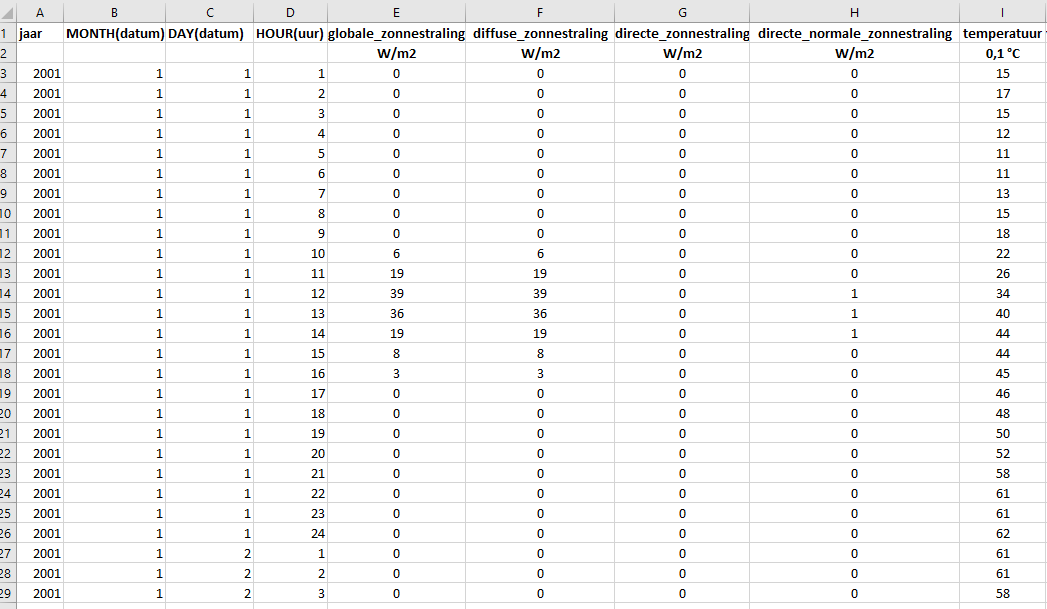
\includegraphics[width=.8\linewidth]{Pictures/NEN5060.png}  
		\caption{NEN 5060 spreadsheet (detail)}
		\label{fig:nen5060}
	\end{subfigure}
	\begin{subfigure}{.3\textwidth}
		\centering
		% include second image
		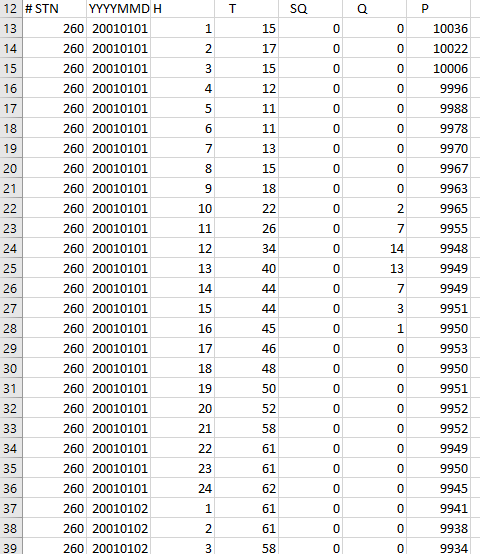
\includegraphics[width=.8\linewidth]{Pictures/KNMI.png}  
		\caption{KNMI hourly data in csv format (detail)}
		\label{fig:knmi}
	\end{subfigure}
	\caption{NEN 5060 spreadsheet and parent KNMI hourly weather record.}
	\label{fig:fig}
\end{figure}


\lstinputlisting[label=lst:nen2pandas, linerange={277-277, 308-328}, 
caption={Conversion of NEN5060 timestamp to timezone-aware Pandas Timestamp}] 
{C:/Data/PROJECTS_NOVA/MCSE@BTO/FUTUREFACTORY/twozone_housemodel-git/housemodel/weather_solar/weatherdata.py}

\subsubsection{Gregorian and Julian time}

Today's calendar is the Gregorian calendar, introduced by pope Gregory XIII in 1582. This calendar refines the use of leap years, compared to its predecessor, the Julian calendar, introduced by Julius Caesar in 45 B.C. \cite{timeanddate}. In the transition process in October 1582, 10 days had to be skipped. It is clear that this time gap was good for society (finally, Turkey introduced the Gregorian calendar in 1926!), but not for astronomy. That is why astronomers kept using the Julian calendar - between 1582 and 1926 - and ever since. That means they have to define a new epoch every 50 years, to compensate for the imperfections of the Julian calendar. The big advantage is that the planets have kept their undisturbed orbits and that the Harmony of the Spheres is still in sync with ancient times.

\subsection{Position of the sun}

\subsection{Attenuation of the solar radiation}

\subsection{Direct Normal Incidence (DNI)}

\subsection{Orientation of the receiving surface}

\subsection{Direct, diffuse and global irradiation}

\subsection{Efficiency}

\newpage